%ब
\section{Experimental API}\label{s:implementation-API}

The experimental \ac{API}\footnote{
The source code is available at \url{http://code.google.com/p/harsha-api/}.
} was designed generically in order to ensure that it
can be used by  applications to maintain dependencies within their keyspaces
irrespective of keyspace schemas or structures of column families.  However,
applications using this \ac{API} still have to supply  the list of referential
integrity constraints as these are not automatically deduced from their
implementation. Instead, the constraints have to be introduced according to the
solution as it is explained in detail in
Section~\ref{s:implementation-MDinSolutions}. 

% Thus,   this \ac{API} is made adaptable to different keyspace schemas  that
% can be deployed in column-oriented key-value \acp{DBMS}.

This \ac{API} validates the referential integrity based on the metadata provided
for the application and its column families.   It  provides the implementation of
all the four solutions as well as the required components to successfully
maintain referential integrity in Cassandra.

The  class diagram of the \ac{API} is presented  in
 Figure~\ref{f:classDiagram} alongside with the  classes that belong to 
the University keyspace example.  The design of the \ac{API} follows the
\ac{ER} model and the main components are the entities, entity managers,  and
validation handlers,  all of which are described in the next sections.
 Notice that for the sake of clarity and brevity,   the class diagram only
 contains  the relevant  methods of the classes,  favoring a simpler
explanation of the functioning of the \ac{API}. 

\begin{landscape}
\begin{figure}[c]
	\centering
	%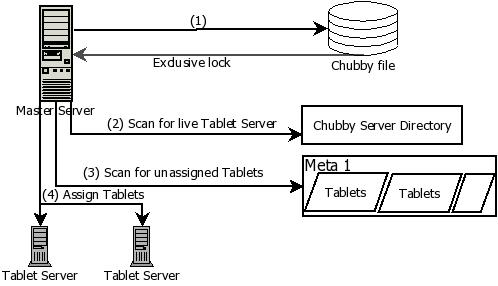
\includegraphics[width=5cm,    height=5cm]{.  /figure/random.  jpg}
% 	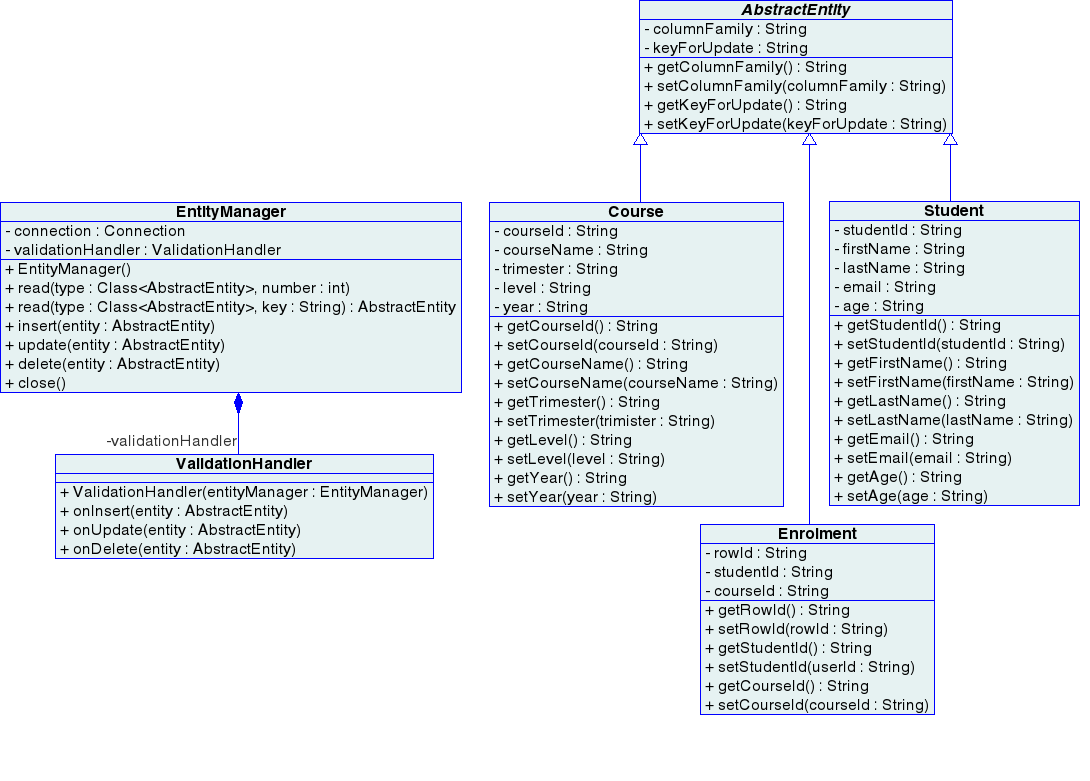
\includegraphics[width=\textwidth]{./figure/Solutions/FinalClassDiagram.png}
	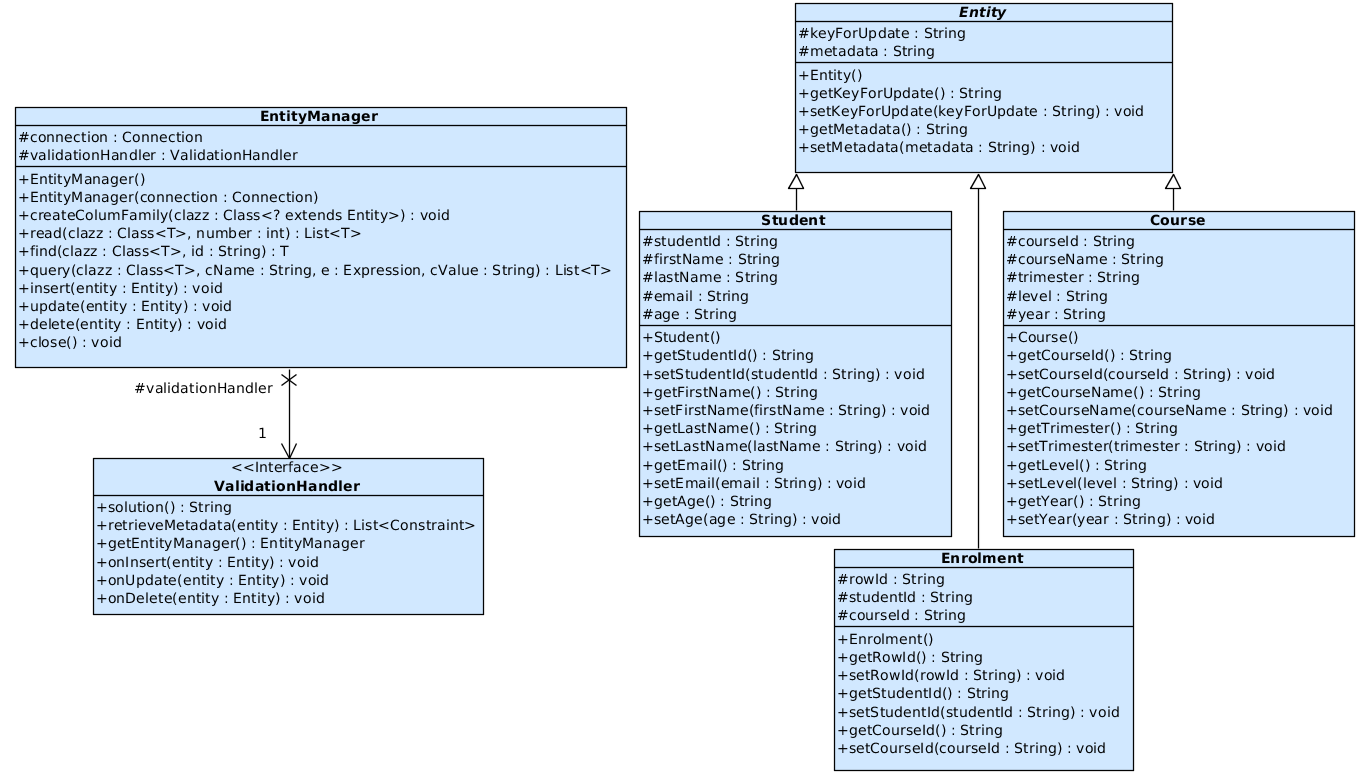
\includegraphics[width=1.45\textwidth]{./figure/uml/class-diagram.png}
	\caption{Class Diagram for the \ac{API}}\label{f:classDiagram}
\end{figure}
\end{landscape}

	\subsection{Entities} 
	
	An \texttt{Entity} class contains attributes (with respective getters and
	setters) that map to columns within a specific column family.  As such,  the contents of a
	column family can be represented by a list of entity objects.  All entities in
	the \ac{API} extend from the class \texttt{Entity}  to
	aid the \ac{API} towards their management.  Particularly,  the attributes
	that \texttt{Entity} contains  are \texttt{columnFamily} which
	determines the column family to which the entity maps,  and 
	\texttt{keyForUpdate} which shall contain the new value in case the primary key
	of the entity is to be updated. 
	
	For example,   considering the University keyspace example,  \texttt{Enrolment} 
	is an entity class that  maps to the \texttt{Enrolment}  column family,  thus
	containing the attributes \texttt{RowId},  \texttt{CourseId} and
	\texttt{StudentId} which represent its respective columns.  As such,  an
	instance of \texttt{Enrolment} contains the values of one super column.  Likewise, 
	\texttt{Student} and \texttt{Course} are entity classes and their instances 
	map to   super columns in their respective column families. 
% 	For all the solutions in this \ac{API},   entities of the user applications are
% 	designed to extend the abstract class called \texttt{Entity},   which has
% 	information about the  methods for accessing and defining  entities.   For
% 	every column family,  applications derive a class from the
% 	\texttt{Entity} containing attributes. 
	Thus, the \ac{CRUD} operations that are performed on these entities  and are
	handled by the \texttt{EntityManager} class, explained next. 
		 
	\subsection{EntityManager} \label{ss:Implementation-API-EntityManager}

	The  \texttt{EntityManager} class implements  all
	the \ac{CRUD} operations to be performed on the entities.  In order to perform
	these operations,   the \texttt{EntityManager} interacts with the respective
	keyspace the entity belongs.  Moreover,  it ensures to trigger the   referential
	integrity validation process whenever a \ac{CRUD} operation requires it. The
	validation is triggered by invoking the respective methods on the  
	\texttt{ValidationHandler} object which is contained within the
	\texttt{EntityManager}.
	
	The \texttt{EntityManager},  before performing any operation,  requires a
	connection to the keyspace.  This connection is established using a third-party
	\ac{API} named Hector~\citep{hector}.  Hector  encapsulates the driver-level
	interface provided by Cassandra (known as Thrift) and simplifies the interaction
	with it.  Regarding the \ac{CRUD} operations,  Hector provides  a
	\texttt{Mutator} class that  encapsulates the necessary procedures to
	create, update, and delete \todo{a record}, and different classes to query
	for data (e.g. \texttt{SliceQuery}).
	 
	 Notice that  the \texttt{EntityManager} is able to generically deal with any
	 entity that derives from the \texttt{Entity} class. This can be seen in the
	 class diagram where \texttt{T} is a generic type which extends \texttt{Entity} 
	 and is used across the \ac{CRUD} methods. The \texttt{EntityManager} is able
	 to deal with any entity by using reflection, a Java
	 feature that performs  an introspection of a class to retrieve its
	 attributes, methods, annotations, among others. Moreover, the
	 methods retrieved from such a class can be invoked on an object in run-time. 
	 Thus, the \texttt{EntityManager} uses reflection to invoke the respective 
	 getter and setter methods of an entity in order to load it with data
	 from the column family or to write the data into a column family.
	 
	 
	
% 	Hector is a high
% 	 level client that wraps the driver-level interface of Cassandra called Thrift. 
% 	 Hector  provides some features that  Thrift does not,  for example,  
% 	 fail-over mechanisms and connection pooling (\todo{cite book}).   
	 % 	 While there
% 	 are other wrappers for Thrift,  Hector was  chosen as  it is one of the
% 	 earliest wrappers and  encapsulates the interaction with the Thrift \ac{API}
% 	 and makes it simpler to access a Cassandra cluster. 	
	
	
	
	
		\subsubsection{Create}
		
		The \texttt{create} (or \texttt{insert}) operation stores an entity in its
		respective column family. This operation triggers a referential integrity
		 validation whenever an  entity is  inserted.  Such validation is performed by
		 the \texttt{onInsert} method of \texttt{ValidationHandler}.
		  Finally, if the
 		 \texttt{ValidationHandler} allows it,  the \texttt{EntityManager} passes the
		  entity details  including row key and column family as parameters to the
		 \texttt{addInsertion} method of the Hector \texttt{Mutator} object to perform
		 the insertion. This operation is detailed in Algorithm~\ref{a:em:insert}
		 
		 
		 
		 		 \begin{algorithm}[h]
		 	\small
		 	\caption{Insert algorithm in \texttt{EntityManager}}\label{a:em:insert}
% 			\SetKwInOut{Input}{input}\SetKwInOut{Output}{output}
			\SetKwFunction{onInsert}{onInsert}
			\SetKwFunction{addInsertion}{addInsertion}
			\SetKwFunction{execute}{execute}
			\SetKwData{e}{e} 
% 			\SetKwData{validationHandler}{validationHandler}
			\KwIn{\texttt{Entity} \e to insert}
			\Begin{
				invoke \onInsert on validationHandler passing entity \e ;\\
				
				\If{no exception is thrown}{
					retrieve the attributes of \e;\\
					\ForEach{attribute}{
						invoke \addInsertion on Mutator passing attribute;\\
					}
					invoke \execute on Mutator;\\
				}			
			}
			
		 \end{algorithm}
% 		For example, all the student entities are inserted into the column family
% 		\texttt{Student} through the \texttt{EntityManager}.  
		

			
		\subsubsection{Read}
		The  \texttt{read} operation retrieves  entities from the column family mapped
		by the entity class.		
		This \ac{API} provides three methods for retrieving entities: \texttt{find},
		\texttt{query} and \texttt{read}. The \texttt{find} method retrieves a single
		entity given the class and the value of its primary key. The \texttt{query}
		method retrieves a list of entities from a column family given the class and a
		conditional expression $\left(< \;,\; \leq\;,\;=\;,\;\geq\;,\; > \right)$ on a
		column name and and its column value. The \texttt{read}  method retrieves
		 the list of entities contained in the column family. These methods are
		 detailed in Algorithms~\ref{a:em:find}, \ref{a:em:query} and~\ref{a:em:read},
		 respectively.  
		 
		 Notice that, these   operations do not prompt any referential
		  integrity validation since entities are only read and their state is not
		 changed,  unlike in the other operations.
		  
		  \begin{algorithm}[h]
		  	\caption{Find algorithm in \texttt{EntityManager}}\label{a:em:find}
		  	\small
			
		  	\KwIn{\texttt{Class<T extends Entity>} clazz, \texttt{String} value }
		  	\KwResult{\texttt{<T extends Entity>}}
		  	
		  	\Begin{
		  		retrieve attributes of clazz;\\
		  		create \texttt{SliceQuery} of clazz where PK = value;\\
		  		\If{no result is found}{
		  			\Return null;
		  		}\Else{
		  			create instance of clazz;\\
		  			load instance with result;\\
		  			\Return instance;
		  		}
		  		 
		  	}
		  	
		  \end{algorithm}

		 \begin{algorithm}[h]
		  	\caption{Query algorithm in \texttt{EntityManager}}\label{a:em:query}
		  	\small
			
		  	\KwIn{\texttt{Class<T extends Entity>} clazz, \hspace{\textwidth} 
		  	\texttt{String} columnName,
		  	\texttt{Expression} expression, \texttt{String} columnValue}
		  	\KwResult{List of \texttt{<T extends Entity>}}
		  	
		  	\Begin{
		  		retrieve attributes of clazz;\\
		  		create \texttt{IndexedSlicesQuery} of clazz where\\ \hspace{1cm}columnName
		  		expression columnValue;\\
		  		\ForEach{result found}{
		  			create instance of clazz;\\
		  			load instance with result;\\
		  			add instance to list;\\ 
		  		}
		  		\Return{list} 
		  	}
		  \end{algorithm}
		  
		  \begin{algorithm}[H]
		  	\caption{Read algorithm in \texttt{EntityManager}}\label{a:em:read}
		  	\small
			
		  	\KwIn{\texttt{Class<T extends Entity>} clazz}
		  	\KwResult{List of \texttt{<T extends Entity>}}
		  	
		  	\Begin{
		  		retrieve attributes of clazz;\\
		  		create \texttt{RangeSlicesQuery} of clazz\\
		  		\ForEach{result found}{
		  			create instance of clazz;\\
		  			load instance with result;\\
		  			add instance to list;\\ 
		  		}
		  		\Return{list} 
		  	}
		  \end{algorithm}

		
		
		\subsubsection{Update}\label{ss:update}
		
		The \texttt{update} operation changes the columns of an existing entity. If
		the changes to be performed are on columns which are not the primary key, then
		an \texttt{insert} operation is performed as it uses the primary key value of
		the entity to locate and replace the column values. Otherwise, if the
		primary key value is to be updated, then more actions need to be performed.
		Firstly, the entity with new primary key value has to be inserted, then all
		the children entities have to be located and their foreign keys updated to
		reflect the new primary key value, and finally the old entity has to be
		removed. 
		
		This operation triggers referential integrity constraints which are
		validated by the method \texttt{onUpdate} of the \texttt{ValidationHandler}
		when the primary key value is to be updated, otherwise, the respective
		validations are performed when the entity is inserted. 
		
				
			\begin{algorithm}[h]
			\caption{Update algorithm in \texttt{EntityManager}}
			\small
			\SetKwFunction{onUpdate}{onUpdate}
			\SetKwFunction{KwInsert}{insert}
			\SetKwFunction{delete}{delete}
			\SetKwData{e}{e}
			
			\KwIn{\texttt{Entity} \e to update}
			\Begin{
				\If{primary key value of \e is not changed}{
					invoke \KwInsert on this \texttt{EntityManager} passing \e;\\
					\Return{}	
				}
				
				\KwInsert entity with \texttt{keyForUpdate} as primary key;\\
				
				invoke \onUpdate on validationHandler passing entity \e ;\\
				
				\If{no exception is thrown}{
					invoke \delete from this \texttt{EntityManager} passing \e;\\
				}\Else{
					\delete entity with \texttt{keyForUpdate} as primary key;\\
				}
			}
		\end{algorithm}
% 		
% 		
% 		
% 		\subsubsection{Update}\label{ss:update}
% 		The \texttt{update} operation perform changes to an existing \todo{record}
% 		 an entity and with new .
% 		  
% 		
% 		 to the contents of
% 		an entity with new contents and .   In other words,  the  values of the columns an entity
% 		represents are updated to new values and committed into the column families.
% 		
% 		The \texttt{EntityManager} provides the following three types of updates. 
% 		
% 		
% 		\begin{description}
% 			\item [Case A: Update Primary Key]  where the attribute
% 			\texttt{keyForUpdate} is used to indicate the change in the primary key.
% 			Before the primary key is updated, and there are child dependencies referencing
% 			the primary key,  the following steps are performed to complete the
% 			\texttt{update} operation.
% 		% In order to do so,  the \texttt{EntityManager} passes the entity to the
% 		% \texttt{ValidationHandler}  to check for referential integrity,  retrieves the
% 		% list of child entities that depend on its primary key,  deletes dependencies
% 		% and the entity,   and update the dependencies Following this,  the steps that
% 		% are performed are :
% \todo{FIX}
% % 			\begin{enumerate}
% % 			  
% % 			  
% % 			\item Check with the \texttt{ValidationHandler} if the entity can be updated.
% % 		
% % 			
% % 			\item Set the primary key of the entity to the \texttt{keyForUpdate} value. 
% % 			
% % 			\item Perform an \texttt{insert} of the entity with the new primary key.
% % 			
% % 			\item Retrieve the list of any child entities that depend on the old primary key
% % 			of the entity.
% % 
% % 			\item Update the foreign keys of the list of child entities to match the value
% % 			of the new primary key of the entity.
% % 			
% % 			\item Perform a \texttt{delete} operation on the old entity.
% % 		\item
% % 
% % 			\end{enumerate}
% % 		
% 		
% 	
% % 		In all the solutions,   an \texttt{Update} operation triggers a referential
% % 		 integrity validation whenever any primary or foreign keys of any entities are
% % 		updated. 
% % 		The validations are performed by the \texttt{onUpdate} method of the
% % 		\texttt{ValidationHandler}. 
% 			If the update is not a cascaded one, the child entities are not updated to
% 			the new primary keys. This is explained in Section~\ref{} Notice that such a
% 			procedure is used to circumvent the restriction of Cassandra to change a primary key.  Once a record has been
% 			inserted into the column family,  the primary key cannot  be changed.  This is
% 			known as a tombstone delete,  which prevents deleting a primary key or
% 			changing it. 
% 		
% 		
% 		
% 			\item [Case B: Update  Foreign Key]  where  the \texttt{ValidationHandler}
% 			is used to check if the foreign keys can be updated and
% 			the respective getter and setter methods of the entity are used to perform the
% 			changes. 
% 			
% 			\item [Case C: Update Attributes]  where a normal update takes place as long as
% 			the attributes  are not keys or referenced anywhere.
% 			
% 		\end{description}
		
		
% 		one in which ,   another in which the foriegn keys are changed
% 		and lastly the one in which attributes that are not keys or referenced anywhere
% 		are changed.  In the former case,  the attribute \texttt{keyForUpdate} is used to
% 		indicate the change in the primary key.  In the case where forieng keys are
% 		updated,   respective getter and setter methods of the  entity are used to
% 		perform the changes.  In both these cases,  referential
% 		integrity needs to be ensured. 
% 		
% % 		it uses the primary key of the entity to update it,  and the other one in which
% % 		uses the especial field \texttt{keyForUpdate} to update the primary as well as
% % 		the rest of the fields. 
% 		 
% 		When the entity to be updated does not contain a change in its keys,  a normal
% 		update takes place using its getter and setter methods.   
		
		
		\subsubsection{Delete}\label{ss:delete}
		The  \texttt{Delete} operation removes  an entity from its respective column
		family.  As mentioned before,  primary key values  will never cease to exist
		in Cassandra due to the tombstone delete, hence, this operation
		empties the values of the columns represented within the entity to be deleted.
		Even when primary key values exist within the column families for deleted
		entities, these are ignored on \texttt{read} operations.
		
		The \texttt{Delete} operation triggers referential
		integrity validations every time an entity is deleted.  
		 This validation is performed by the \texttt{onDelete} method of the
		 \texttt{ValidationHandler}.  Finally,  if the
		\texttt{ValidationHandler} allows it, the \texttt{EntityManager} passes the
		 necessary information to the \texttt{delete} method of the Hector
		 \texttt{Mutator} object. This operation is detailed in
		 Algorithm~\ref{a:em:delete}.
 		
 		\begin{algorithm}[H]
			\caption{Delete algorithm in \texttt{EntityManager}}\label{a:em:delete}
			\small
% 			\SetKwInOut{Input}{input}\SetKwInOut{Output}{output}
			\SetKwFunction{onDelete}{onDelete}
			\SetKwFunction{delete}{delete}
			\SetKwData{e}{e} 
			
			\KwIn{\texttt{Entity} \e to delete}
			\Begin{
				invoke \onDelete on validationHandler passing entity \e ;\\
				
				\If{no exception is thrown}{
					retrieve attributes  of \e;\\
					invoke \delete on Mutator passing primary key  and column family
					of \e;\\
				}			
			}
			
		\end{algorithm}
		
 		
%  		Before a parent entity is deleted,  the \texttt{EntityManager} retrieves the
%  		child entities it depends upon  from he \texttt{ValidationHandler} if the
%  		 referential intergity is not violated.  The \texttt{EntityManager} deletes
%  		the child entities prior to deleting the parent entity. 
		
		
		
		
		\subsection{ValidationHandler}\label{ss:VH}
		The \texttt{ValidationHandler} is used by the \texttt{EntityManager} every time
		an operation triggers  referential integrity validations on any entity.
		It contains the  logic that  checks  if an entity has dependencies,
		verifies whether the \texttt{insert}, \texttt{update} or
		\texttt{delete} operations performed on an entity  violate  referential
		integrity constraints, and it also applies referential integrity rules
		when operations are cascaded or updates nor deletes are allowed. 
		
		
% 		 In order to ensure that these operations maintain referential integrity
% 		  between entities,  it applies the appropriate referential integrity rules
% 		 explained in Section~\ref{s:referential-integrity}. Similarly,  for
%  		\texttt{update} and \texttt{delete} operations their respective rules are
%  		applied.   The referential integrity validation performed by the
% 		\texttt{ValidationHandler} for each of these operations is discussed next.
		
		The \texttt{ValidationHandler} is just an interface that has to be implemented
		to deal with each solution. However, since the validations are the same across
		solutions, it is sufficient to provide a generic
		class that implements the \texttt{ValidationHandler} for \ac{CRUD} operations.
		Thus, it is left for each solution to extend the generic
		\texttt{ValidationHandler} and just implement the \texttt{retrieveMetadata}
		method accordingly.
		
% 		Notice that, the \texttt{ValidationHandler} has access to the
% 		\texttt{EntityManager} in order to look-up for dependencies and metadata of an entity as soon as  validation is
% 		invoked on an entity.
% The \texttt{EntityManager} passes the entity and the connection details  to
% the \texttt{ValidationHandler} to perform the validation.
		
		
		
	
	\subsubsection{Validation: \texttt{onInsert}}
		This validation is triggered every time the \texttt{EntityManager} is asked to
		insert an entity. It occurs before the insertion of the actual data as the
		validation has to check whether the entity has foreign keys to other column
		families. This is determined by retrieving the  constraints relevant to the
		entity, and if a constraint indicates that the entity has foreign keys,
		this validation must ensure that they match the primary keys of the
		respective column families they reference. This validation is detailed in
		Algorithm~\ref{a:vh:onInsert}.
	
	 	\begin{algorithm}[H]
	 		\caption{Validation \texttt{onInsert}}\label{a:vh:onInsert}
	 		\small
	 		\SetKwData{e}{e}
	 		\SetKw{throw}{throw}
	 		\KwIn{\texttt{Entity} e to be inserted}
	 		\Begin{
	 			retrieve the metadata of \e;\\
	 			\ForEach{constraint of type \texttt{R} $\in$ metadata}{
					retrieve referenced constraint \texttt{RConstraintName};\\
					determine the entity class that maps to the parent column family;\\
					use \texttt{EntityManager} to find parent entity;\\
					\If{parent entity does not exist}{
						\throw Exception;\\
					}
	 			}
	 		}
	 	\end{algorithm}
	 	
	 	
For example,  when an \texttt{Enrolment} entity is to be inserted,   the
 \texttt{Validation\-Handler} identifies the parent column families  by looking up
 at the \ac{FK} constraints of the entity. In this case, there
 is only \texttt{CONST400} which identifies \texttt{Student} as a parent column
 family. Hence, the \texttt{ValidationHandler} makes sure there is a
 \texttt{Student} entity whose primary key value matches the foreign key value
 of the \texttt{Enrolment} entity to be inserted. If such a parent entity
 exists, then the \texttt{EntityManager} is allowed to \texttt{insert} the entity.
		
		
	\subsubsection{Validation: \texttt{onUpdate}}
		This validation is triggered every time the \texttt{EntityManager} is asked to
		update an entity which primary key value has changed. Recall that if the changes
		of the entity to  be updated do not involve the primary key, then an
		\texttt{insert} takes place instead and hence the validation is performed by
		\texttt{onInsert}. Otherwise, if the primary key value of the entity is changed,
		the new entity is  inserted, the foreign keys of the dependencies are updated to
		the new primary key value, and the old entity is deleted. Clearly, the
		referential integrity rules apply in this validation. These are assumed to be
		contained within the  \texttt{DeleteRule}\footnote{Notice that for the sake of
		simplicity, this rule is also used for update operations} field of the
		constraints relevant to the children entities.  Thus, the validation finds all
		the child dependencies of the entity and, if the \texttt{DeleteRule} is
		\texttt{CASCADE}, updates their corresponding foreign keys to the new primary
		key value. Otherwise, if the \texttt{DeleteRule} is \texttt{NODELETE}, the
		update is only allowed if there are no child dependencies. Notice that this
		operation assumes the entity with new primary key value has already been
		inserted. This validation is detailed in Algorithm~\ref{a:vh:onUpdate}.
		
		\begin{algorithm}[h]
			\caption{Validation \texttt{onUpdate}}\label{a:vh:onUpdate}
			\small
	 		\SetKwData{e}{e}
	 		\SetKw{throw}{throw}
	 		\KwIn{\texttt{Entity} e to be updated}
	 		\Begin{
	 			retrieve the metadata of \e;\\
	 			\ForEach{constraint of type \texttt{F} $\in$ metadata}{
					retrieve referenced constraint \texttt{RConstraintName};\\
					\If{\texttt{DeleteRule} is \texttt{CASCADE}}{
						determine the entity class that maps to the child column family;\\
						use \texttt{EntityManager} to query for the children of \e;\\
						add children to list;\\
					}\ElseIf{\texttt{DeleteRule} is \texttt{NODELETE}}{
						determine the entity class that maps to the child column family;\\
						use \texttt{EntityManager} to query for the children of \e;\\
						\If{\e has children}{
							\throw Exception;
						}
					}
	 			}
	 			\ForEach{child $\in$ list}{
	 				use \texttt{EntityManager} to update child;
	 			}
	 		}
		\end{algorithm}
		
		
		
For example,   in the University keyspace,   if the primary key of a 
		\texttt{Course} entity is to be updated,    the \texttt{ValidationHandler}
locates the \ac{FK} constraints which reference \texttt{Course}. In this case,
only \texttt{CONST600} references \texttt{Course}, which follows up to
\texttt{CONST500} from which the child entity can be retrieved.
Since the \texttt{DeleteRule} is \texttt{NODELETE}, it is checked if there are
any \texttt{Enrolment} entities which reference the course to be updated. If
there are child entities, an exception is thrown and the update of the
\texttt{Course} entity is not allowed. Otherwise, if no \texttt{Enrolment}
entities refer to such a course, the \texttt{EntityManager} is allowed to update
its primary key value.
		
		
	\subsubsection{Validation: \texttt{onDelete}}
		This validation is triggered every time the \texttt{EntityManager} is asked 
		to delete an entity. This validation ensures that referential integrity rules
		are applied when the entity is referenced by other entities. That is, the
		entity to be deleted is parent of other entities. The referential integrity
		rule to apply can be \texttt{CASCADE} or \texttt{NODELETE}. In the former
		case, child dependencies on the entity are deleted, while deletion in the
		latter case is only allowed when the entity has no child dependencies. This
		validation is detailed in Algorithm~\ref{a:vh:onDelete}.
		
		
		
		For example,   in the University keyspace,   if a 
		\texttt{Student} entity is requested to be deleted,    the
		\texttt{ValidationHandler} locates the \ac{FK} constraints which reference \texttt{Student}. In this
		 case, only \texttt{CONST700} references \texttt{Student}, which follows up
		 to \texttt{CONST400} from which the child entity can be retrieved.
		Since the \texttt{DeleteRule} is \texttt{Cascade},  
		the child entities are deleted from \texttt{Enrolment} and no exception
		is thrown, hence allowing the \texttt{EntityManager} to  delete the
		entity from its \texttt{Student} column family.
	
		\newpage
		\begin{algorithm}[H]
	 		\caption{Validation \texttt{onDelete}}\label{a:vh:onDelete}
	 		\small
	 		\SetKwData{e}{e}
	 		\SetKw{throw}{throw}
	 		\KwIn{\texttt{Entity} e to be deleted}
	 		\Begin{
	 			retrieve the metadata of \e;\\
	 			\ForEach{constraint of type \texttt{F} $\in$ metadata}{
					retrieve referenced constraint \texttt{RConstraintName};\\
					\If{\texttt{DeleteRule} is \texttt{CASCADE}}{
						determine the entity class that maps to the child column family;\\
						use \texttt{EntityManager} to query for the children of \e;\\
						add children to list;\\
					}\ElseIf{\texttt{DeleteRule} is \texttt{NODELETE}}{
						determine the entity class that maps to the child column family;\\
						use \texttt{EntityManager} to query for the children of \e;\\
						\If{\e has children}{
							\throw Exception;
						}
					}
	 			}
	 			\ForEach{child $\in$ list}{
	 				use \texttt{EntityManager} to delete child;
	 			}
	 		} 
	 	\end{algorithm}
		
		\begin{comment}
		
		
		
		
		\subsection{ValidationHandler}\label{ss:VH}
		The \texttt{ValidationHandler} is used by the \texttt{EntityManager} every time
		an operation triggers  referential integrity validations on any entity.
		The \texttt{ValidationHandler} has access to the \texttt{EntityManager} in order
		to look-up for dependencies and metadata of an entity as soon as  validation is
		invoked on an entity.
% The \texttt{EntityManager} passes the entity and the connection details  to
% the \texttt{ValidationHandler} to perform the validation.
		
		The \texttt{ValidationHandler} contains the  logic for checking whether an
		entity has any dependencies and verifies whether  \texttt{insert},
		\texttt{update} or \texttt{delete} operations  violate  referential integrity or
		not.   In order to ensure that these operations maintain referential integrity
		between entities,  it applies the appropriate referential integrity rules
		explained in Section~\ref{s:referential-integrity}. Similarly,  for
		\texttt{update} and \texttt{delete} operations their respective rules are
		applied.   The referential integrity validation performed by the
		\texttt{ValidationHandler} for each of these operations is discussed next.
		
	\begin{description}
	\item[onInsert:]
		In an \texttt{insert} operation,  a referential integrity validation is
		triggered before an entity is  inserted. The \texttt{ValidationHandler}  checks
		whether the entity has foreign keys and, if so, whether these refer to valid
		parent entities. That is,  it ensures that the foreign keys of the entity to
		insert match primary keys.  Otherwise, an exception is raised stating that the
		referential integrity has been violated. The following checks are performed by
		the \texttt{ValidationHandler}.
		
		\renewcommand{\labelenumii}{\arabic{enumi}. \arabic{enumii}}
		\renewcommand{\labelenumiii}{\arabic{enumi}. \arabic{enumii}. \arabic{enumiii}}
		
		\begin{enumerate}
		\item If the entity has no \ac{FK} constraints
				\begin{enumerate}
		  		\item \texttt{EntityManager} inserts the entity. 
		  		\end{enumerate}
				
		\item Else,  if the entity has \ac{FK} constraints 
		  		\begin{enumerate}
				\item Identify the parent entity class from the \ac{FK} constraint. 
				\item If foreign keys exist as  primary key in the parent entity class
				  		\begin{enumerate}
				  		\item \texttt{EntityManager} inserts the entity. 
				  		\end{enumerate}
				\item Else
				   		\begin{enumerate}
				   		  \item Raise exception. 
				   		\end{enumerate}
				\end{enumerate}   	
		\end{enumerate}
		The implementation of the \texttt{insert} operation is consistent across all the
		solutions.  
		
	\item[onUpdate:] 
		In an \texttt{update} operation,  a referential integrity validation is
		triggered before the state of an entity is changed.  The validation for an
		\texttt{update} operation is different according to whether primary keys,
		foreign keys or just regular attributes are updated.
		
		\begin{description}
		\item[Case A: Update Primary Key] When a  primary key of a
		parent entity is updated,  the \texttt{ValidationHandler} performs the
		following checks. 
		\renewcommand{\labelenumii}{\arabic{enumi}. \arabic{enumii}}
		\renewcommand{\labelenumiii}{\arabic{enumi}. \arabic{enumii}. \arabic{enumiii}}
		%\renewcommand{\labelenumiiii}{\arabic{enumi}. \arabic{enumii}. \arabic{enumiii}. \arabic{enumiiii}}
		\begin{enumerate}
		  \item If the entity has no \ac{FK} constraints 
		  	\begin{enumerate}
		  		  \item \texttt{EntityManager}  updates the entity. 
			\end{enumerate}		  	
		  \item Else if the entity has  \ac{FK} constraints  
		  		\begin{enumerate}		  	
				  \item If the \texttt{DeleteRule} for the \ac{FK} constraint is
				  \texttt{Cascade}
				    	\begin{enumerate}
				    	  \item Use \texttt{EntityManager} to
				    	   update the primary key of the entity and the foreign keys of the
				    	   child entities. 
						\end{enumerate}
				  \item Else,  if the \texttt{DeleteRule}  is
				  \texttt{NoDelete}\footnote{{Notice that \texttt{DeleteRule} is considered as the rules applied on
				  \texttt{update} operations for brevity and simplicity.}}
						\begin{enumerate}
						  \item If the entity has no child entities,  
% 						  		\begin{enumerate}
						  		   \texttt{EntityManager}  updates the entity. 
% 						  		\end{enumerate}
						  \item Else,  if the entity has child entities,  
% 						   		\begin{enumerate}
						    	  Raise exception.  
% 						    	\end{enumerate}
						\end{enumerate}
				\end{enumerate}
		 \end{enumerate}
		 
		For example,   in the University keyspace,   when a
		 \texttt{keyForUpdate} is provided for an existing  \texttt{Student}
		entity,   the \texttt{ValidationHandler}
		checks the metadata and locates the \ac{FK} constraint \texttt{CONST400} as
		seen in Figure~\ref{f:metadataInSolutions}.  Since the \texttt{DeleteRule} is
		\texttt{Cascade},  the \texttt{ValidationHandler} allows the \texttt{update}
		operation to take place as explained in Section~\ref{ss:Implementation-API-EntityManager}. 
			
% 			For example,  when the foreign key \texttt{StudentId} for one of the entities
% 		in \texttt{Enrolment} is given a new value,   then the \texttt{ValidationHandler} 
% 		identifies the parent entity class for its \ac{FK} constraint
% 		\texttt{CONST400} as \texttt{Student}.   If the new \texttt{StudentId} 
% 		exists as a primary key for any
% 		 of the  entities in \texttt{Student} entity class,   the \texttt{update} is
% 		 performed. 
		 % \acresetall
% %ब
\chapter{Experimental Design}

\todo{Check number of enrolments, introduce all metadata, and retrieve 
details of cassandra cluster from my computer}

The implementation of the four solutions  introduces referential integrity
constraints and validations in Cassandra, which are 
not provided by this \ac{DBMS} at the moment of writing. In order to evaluate
 the performance of these four solutions, experiments are 
  conducted by using the implemented \ac{API} described in
  Section~\todo{Section}.   The goal of the experiments is to determine how
  each solution affects the performance of  Cassandra in \ac{CRUD}
  operations, especifically in those where referential integrity validations are
  triggered (namely Create, Update and Delete).

The experimentation is performed on the example application presented across
chapters: the University keyspace. In such an application, different constraints
are added and allow to test the performance under such different application
requirements. The performance of the  solutions provided for ensuring
referential integrity  is measured based on response time and throughput.

This chapter is structured as follows.
Section~\ref{sexp:BenchmarkKeyspace} describes the example application 
used for the experiments. Section~\ref{sexp:CassandraCluster} provides the
details of the nodes used in the Cassandra cluster. Section~\ref{sexp:ExperimentalSetup}
describes the experimental setup to evaluate the performance of the solutions.
Section~\ref{sexp:PerformanceIndicators} presents the performance indicators
 considered for measuring the results from the experiments. Finally,
Section~\ref{sexp:Summary} presents a summary of the chapter.


\section{Example application} \label{sexp:BenchmarkKeyspace}
% In order to asses the performance of Cassandra when the four solutions are
% executed,
% In the experiments, the experimental \ac{API} is implemented by loading
% entitites belonging to a prototype keyspace designed for these experiments. The
% prototype keyspace is modelled on a University keyspace that stores the details
% of students and courses along with the enrolment details of the students.The
% class diagram for the University keyspace is shown in
% Figure~\ref{fexp:ClassDiagram}. The entities are saved as the following column
% families in Cassandra.

The  \ac{API} designed and implemented in the previous chapters is validated and
tested by performing \ac{CRUD} operations on an example application
especifically designed for this purpose. This application has been referred to
as the \texttt{University} keyspace in previous chapters, and it contains
different constraints in order to  assess the performance of the \ac{API} and
the solutions on each of them. This application stores the details of students and
 courses along with the enrolment details of the students. The class diagram for
 the University keyspace is shown in Figure~\ref{fexp:ClassDiagram}, and each
 entity is saved into its respective column family in a Cassandra cluster.

	\begin{itemize}
	  \item \texttt{Student} stores the  following attributes of students:
	   \texttt{StudentId} (primary key), \texttt{FirstName}, \texttt{LastName},
	  \texttt{Email} and \texttt{Age}.
	  \item \texttt{Course} stores  the following  attributes of courses:
	  \texttt{CourseId} (primary key), \texttt{CourseName}, \texttt{Trimester},
	  \texttt{Level} and \texttt{Year}.
	  \item \texttt{Enrolment} stores the  relationship between
	  students and courses, that is, it stores the courses each student is enrolled
	  into.  The attributes for \texttt{Enrolment} are \texttt{RowId} (primary
	  key), \texttt{StudentId} and \texttt{CourseId}, where \texttt{StudentId}
	  and \texttt{CourseId} are foreign keys.
	\end{itemize}
	
	\begin{figure}[h] \centering
		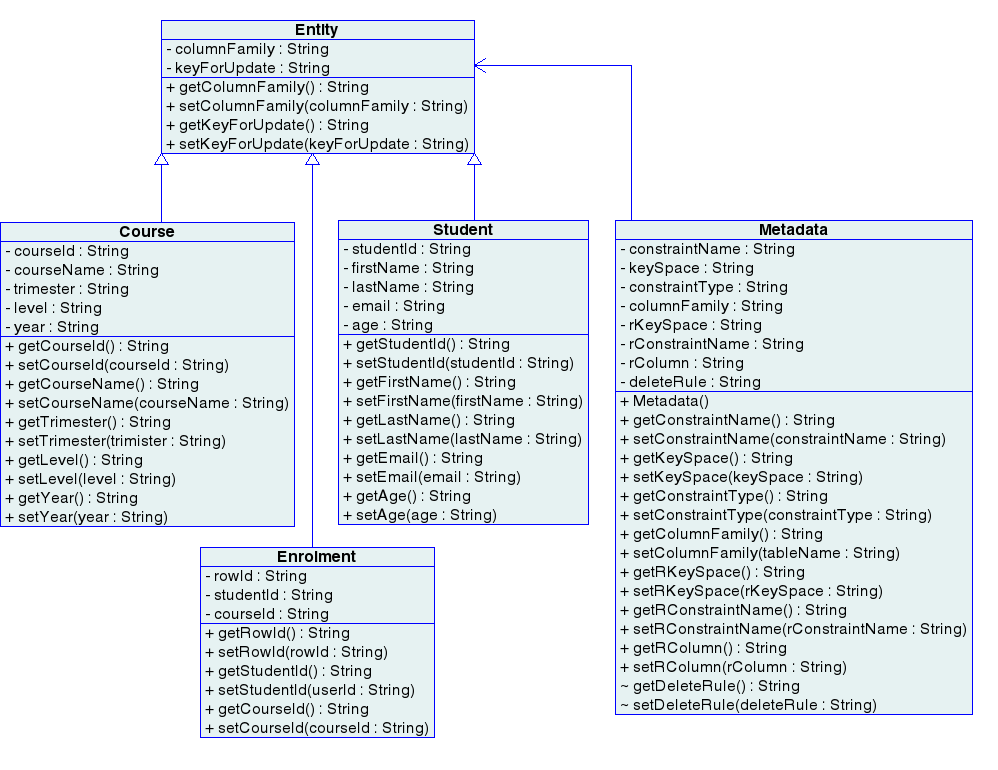
\includegraphics[width=1\textwidth]{./figure/Solutions/classdiagram-experimental.png}
		\caption{Class Diagram for University}\label{fexp:ClassDiagram}
	\end{figure} 

% The constraints for the keyspace are stored in  a  \texttt{Metadata} entity
% class.These constraints are the \ac{PK} and \ac{FK} constraints applicable on each of
% the column families in this keyspace. The list of constraints are the same for
% all the solutions  and are shown in Table~\ref{texp:ListConstraints}.

The list of constraints created for the University keyspace can be seen in
Table~\ref{texp:ListConstraints}. \texttt{CONST100... CONST700} \todo{explain
the purpose of each of them}.


\begin{table}[h] \label{texp:ListConstraints}
\centering
\caption{Metadata}	
	\newcolumntype{C}{@{\hspace{2.5pt}}>{\scriptsize}c@{\hspace{2.5pt}}}
	\begin{tabular}{CCC CCC CC}
		\toprule
		\bfseries ConstraintName & \bfseries Keyspace & \bfseries ConstraintType &
		\bfseries ColumnFamily & \bfseries RKeyspace & \bfseries RConstraintName &
		\bfseries RColumn & \bfseries DeleteRule\\
		\midrule
		CONST100 & University & P & Student & University & & StudentId &\\
		\rc CONST200 & University & P & Course & University & & CourseId &\\
		CONST300 & University & P & Enrolment & University & & RowId &\\
% 		\hline
% 		\hline
		\rc CONST400 & University & R & Enrolment & University & CONST100 & StudentId
		& CASCADE\\
		CONST500 & University & R & Enrolment & University & CONST200 & CourseId &
		NODELETE\\
		\rc CONST600 & University & F & Course & University & CONST500 & CourseId &
		NODELETE\\
		CONST700 & University & F & Student & University & CONST400 & StudentId &
		CASCADE\\
		\bottomrule
	\end{tabular}
\end{table}

% The \texttt{ValidationHandler} in each solution checks these constraints to
% validate referential integrity within this keyspace. The entities are loaded
% generically by the \texttt{EntityManager} for each solution. 
% In the experiment,
% the number of entities inserted for each column family in all the solutions are
% shown in Table~\ref{texp:EntityList}. 
% 	
% 	\begin{table} \label{texp:EntityList}
% 	\centering
% 	\newcolumntype{C} {@{\hspace{2.5pt}}>{\scriptsize}c@{\hspace{2.5pt}}}
% 		\begin{tabular}{CC}
% 			
% 			\toprule
% 			\bfseries ColumnFamily & \bfseries No. of Entities \\
% 			\midrule
% 			Student & 1000 \\
% 			\rc Course & 1000 \\
% 			Enrolment & 10000  \\
% 	% 		\hline
% 	% 		\hline
% 			
% 			\bottomrule
% 		\end{tabular}
% 	\end{table}


\section{Cassandra cluster} \label{sexp:CassandraCluster}
Cassandra is deployed in an homogeneous cluster conformed by 10 nodes. That is,
 all 10 nodes have the same characteristics in software and hardware. These
 nodes emulate a cloud environment in which each node saves
 the data on the local disks of the machines. The characteristics of these nodes
are:


\begin{itemize}
  \item Hardware: \todo{Look on internet the specs of the model}
  	\begin{itemize}
  	  
  	 \end{itemize}
  \item Software: 
  \begin{itemize}
    \item Operating system
    \item Java JDK
    \item Cassandra version
    \item Hector version
  \end{itemize}
\end{itemize}
% Cassandra is deployed in an homogeneous environment The environment to deploy
% cassandra is an homogeneous cluster conformed by 10 nodes. That is, all 10 nodes have the same characteristics in software and
% hardware. These nodes emulate a cloud environment in which each node runs
% Cassandraand saves the data on te local disks of the machines. The
% characteristics of these nodes are:

% 	\begin{table} \label{texp:Nodeconfig}
% 	\centering
% 	\newcolumntype{C} {@{\hspace{2.5pt}}>{\scriptsize}c@{\hspace{2.5pt}}}
% 		\begin{tabular}{CC}
% 			\toprule
% 			\bfseries System configurations\\
% 			\midrule
% 			Linux kernel version & Linux 3.2.4-1-ARCH i686 \\
% 			\rc CPU & Intel(R) Core(TM)2 Duo CPU     E8400  @ 3.00GHz \\
% 			CPU cores & 4  \\
% 			\bottomrule
% 		\end{tabular}
% 	\end{table}
% 
% 
% 
% Linux kernel version: Linux 3.2.4-1-ARCH i686
% 
% CPU: Intel(R) Core(TM)2 Duo CPU     E8400  @ 3.00GHz
% 
% CPU cores: 4


%             total       used       free     shared    buffers     cached
% Mem:          3195       2941        254          0        212       1493

Cassandra configurations:

Version: 0.8.4

Hector Version: 0.8.0-2

Replication strategy:

Partitioner used: Random Partitioner which distrbutes rows in a cluster evenly.
This is the default configuration setting when Cassandra is installed.

The configurations on all the modes are set to the default values in the yaml
configuration file.

The first node is started as a seed node and has the Auto Bootstrap option set
to true. This allows other nodes with this ndoe as its seed to migrate data from
the seed node while data partitioning. For the rest of the nodes tihs options is
set to false.Hinted Handoff is enabled on all nodes.

\begin{itemize}
  \item Hardware
  \item Software
\end{itemize}




%ब
\section{Experimental setup}\label{sexp:ExperimentalSetup}

The experimentation is based on performing \ac{CRUD} operations upon artificial
data created for the University example application. Since it is not a
controlled environment, the experimentation involves performing several runs
where data is inserted, updated, and deleted on the Cassandra cluster. The
environment is not controlled as variables like network latency, parallel
processes in the nodes, and other variables affect the performance.

On each run,  the time required for each operation is recorded in order to assess
its response time for each solution. Additionally,  

 Notice that, each operation on the
artificial data is performed in a batch,   and entities from each column family
are randomly sorted before any operation takes place.  Random sorting is performed in order to
prevent the results to be biased from possible optimization made by Cassandra in
terms of indexes or other criteria. 
		
The artificial data is made up of  students,   courses,  and 
enrolments which is the result of assigning 10 different courses to each
student.  Courses are assigned by dividing the number of courses
into 100 groups of 10 courses each,  and assigning a group for each student. 
Notice that such an assignment involves that X students have the same courses
assigned.  The quantity of records to be inserted for each entity was chosen
considering an overall reasonable time for completing the experimentation of all
solutions. 
		
The format of the artificial data created is as follows.  
	\begin{itemize}
	  
		  \item \texttt{Student} has a
		unit-increasing \texttt{StudentId},  which is merged into the fields \texttt{FirstName}
		 and \texttt{LastName} as "First Name (StudentId)" and "Last Name
		(StudentId)".  \texttt{Email} is composed in a similar way as
		``First. Last@email. (StudentId). com'' and \texttt{Age} is a random number. 
		
		\item  \texttt{Course} has a unit-increasing \texttt{CourseId} which is
		appended to the prefix "COMP".  It also has a composed \texttt{CourseName} as
		in \texttt{Student} (merging id and field).  \texttt{Trimester},  \texttt{Level}
		and \texttt{Year} are randomly generated numbers. 
		
		\item  \texttt{Enrolment} contains a unit-increasing \texttt{RowId},  and the
		respective foreign keys of student and course,  which are \texttt{StudentId}
		and \texttt{CourseId}. 
		
	\end{itemize}

		
The order of the operations performed on the data is as follows.  \textbf{Create}
inserts all the entities for \texttt{Student},  \texttt{Course} and
\texttt{Enrolment}.  \textbf{Update} performs changes on the primary keys of
students and courses,  and on the foreign keys of \texttt{Enrolment} (the one
relative to courses,  specifically).  Finally,  \textbf{Delete} removes all the
\texttt{Student},  \texttt{Course} and \texttt{Enrolment} entities. 
Notice that the primary keys in every column family are different in each run
(create,  update,  delete) in order to avoid introducing biases to the results as
product of the tombstone delete paradigm that Cassandra utilizes.  That is,  since
Cassandra does not completely  remove the primary keys of the inserted entities
(tombstone delete),  reinsertion  using the same primary key might yield faster
times as the key already exists.  After each run,  all column families
(\texttt{Student},  \texttt{Course},  and \texttt{Enrolment}) are emptied and
ready for the next run.   The details  of the \ac{CRUD} operations are explained
further in the following sections. 
		

	
\subsection{Create} The \texttt{Create} operation inserts all the
\texttt{Student},  \texttt{Course} and \texttt{enrolment} entities in that
precise order due to the nature of the referential integrity constraints
presented in Section~\ref{s:ed:ri}.  The time required to insert all of the
entities in their respective column families  is recorded.  In the
\texttt{Student} and \texttt{Course} column families,  \texttt{Create} does not
trigger any referential integrity validation as these entities do not contain
foreign keys. 
Contrarily,  \texttt{Create} on \texttt{Enrolment} triggers foreign key
validation checks on both \texttt{Student} and \texttt{Course} column families. 
		
\subsection{Update} The \texttt{Update} operation is performed after the
creation of all entities. 
First,  an attempt to update the primary key of each \texttt{Course} entity is
made.  This triggers referential integrity validations that result in exceptions
thrown as the \texttt{DeleteRule} for all \texttt{Course} entities is
\texttt{NoDelete}.  Hence,  the times recorded for updating the \texttt{Course}
column family represent the time required to identify a constraint violation and throw
the respective exceptions. 
					
Next,  the \texttt{Enrolment} column family is updated.  In this case,  the
\texttt{CourseId} for each \texttt{Enrolment} entity is changed to a different
one,  ensuring that the distribution of courses and students remains the same. 
The update on the \texttt{Enrolment} column family triggers referential
integrity validation checks to ensure that the course to which every
\texttt{Enrolment} entity is being updated actually exists in \texttt{Course}
column family. 
					
Finally,  the primary key for each \texttt{Student} entity is updated to a new
integer value that previously  never existed in the column family.  Given the
\texttt{Cascade} \texttt{DeleteRule} for \texttt{Student},  this operation
triggers a cascaded update on the
\texttt{Enrolment} column family.  
%  by respectively updating the student foreign
% key,  \texttt{StudentId} in all its existing \texttt{Enrolment} entities. 
All the dependant \texttt{Enrolment} entities of this \texttt{Student} entity
are respectively updated on its foreign key \texttt{StudentId}. 
		
\subsection{Delete} The deletion of entities occurs first on the
\texttt{Enrolment} column family,  where all of its records are deleted without
requiring referential integrity checks as this is a child entity.  The times are
recorded for each \texttt{Delete} operation and then all of the entities are
reinserted with the same primary keys in order to assess the cascaded delete of
\texttt{Student} entities next. 
				
Secondly,  all  the \texttt{Student} entities are deleted from the
\texttt{Student} column family.  Given the \texttt{Cascade} \texttt{DeleteRule} of these entities,  the
\texttt{ValidationHandler} ensures to delete first all of the child entities
before deleting a \texttt{Student} entity. 
Hence,  the times recorded for this operation measure the time required for
performing a cascaded delete on the student dependencies in enrolment.  Notice
that the dependencies exist at this point as they will have been reinserted into
\texttt{Enrolment} in the previous step. 
				
Finally,  all the \texttt{Course} entities are deleted.  Despite the courses
having a \texttt{NoDelete} rule,  notice that at this point the
\texttt{Enrolment} column family is empty,  so courses can be deleted as there
are no child dependencies.  Thus,  the times recorded for this operation measure
referential integrity validation as well as the \texttt{Delete} operation
of the respective entity.  After this final operation,  all column families are
emptied but all the primary keys still exist due to Cassandra's tombstone
delete.  However,  the whole keyspace is ready for the next batch of operations as
the primary keys of all column families will be different. 
	
	



%ब
\section{Performance Indicators} \label{sexp:PerformanceIndicators}
% Performance of database systems is commonly measured in terms of the
% \textit{Response time} and \textit{Throughput}. 

In this thesis,  response time and throughput are the measures used to gauge the
performance of the four solutions while referential integrity validation is
implemented using the \ac{API}. 
Response time refers to the time  a database system takes to process an
operation and produce results to the end user(\todo{cite Demurjian, 
Berkely, serverside, }).  
% Measuring response time for a
% database operation is similar to a black-box evaluation because it is measured 
% without considering the internal functioning  of the database system.  According
% to (\todo{cite Demurjian}) such an evaluation is ideal for a complete database
% system to measure its performance and to give the users details about its 
% efficiency and speed in performing operations.  
Response time for each of the  operations that trigger such a validation from
all the solutions are measured during the experiments. 
This included the time involved to access and retrieve metadata for the entities
and also the time for validating referential integrity by the
\texttt{ValidationHandler}.  
% The response time of Cassandra when such validations
% are not in place is also measured and considered as a baseline with which to
% analyse the solutions.  Such a comparison determines the degree of change in
% speed of Cassandra when such overheads are introduced and gives users useful
% information about how each solution affects the performance of the database
% system. 

The second performance measure used is \textit{Throughput} which is another
classical and commonly used measure of database performance (\todo{cite
BerkleyDB}).  Throughput measures the number of operations processed by the
database system in a unit of time.  In the experiments the throughput of all the
operations triggering referential integrity validation across all solutions is
measured as operations per second.  A single operation stands for each time an
entity is inserted or updated or deleted. Note that only the operations that
introduce the referential integrity validation are measured and thus
\texttt{read} operations are not measured in terms of response time or
throughput. 

% For example,  inserting 1000 students means that 1000 \texttt{insert}
% operations are processed by Cassandra. 
Notice that external variables such as network latency,  simultaneous processes
in the operating systems of each node,  and other variables are not considered
for the analysis of results.  Even when they are present,  it is expected that
results will not be biased by them.  Nonetheless,  the experiments will be
performed at night time over weekends as this is the time when the cluster is
least used,  thus reducing the presence of such variables and hence their impact
by biasing the results. 

In the experiments,  response time and throughput are measured by logging the
time involved to complete each operation in all the solutions. 
For this,  the  real time is recorded before and after every validation.  When all
the iterations of the experiment are completed,  the time
measurements are written to an output log file. 

The traditional TPC benchmarks are not considered as performance measures in
this experiment  because these benchmarks are centred around transactions and
OLTP workloads.  The principal metrics for these benchmarks are the transaction
rate,  query per hour,  cost indicators of a system,  among others,  which are
suitable indicators for \ac{DBMS} with ACID properties~\citep{TPC}.  Hence,  for
assessing Cassandra which lacks SQL queries and  ACID properties,  these
benchmarks are not suitable indicators of performance. 
%  it is
% essential to measure it in terms of what is critical to application  using Cassandra.  In this experiment it is critical to
% measure the difference in time for an operation to complete in Cassandra when
% referential integrity validation is activated or not activated. 


% These operations which trigger referential integrity validation for an entity
% namely the \texttt{insert},  \texttt{update},  \texttt{delete} operations are
% were measured in terms of the throughput in the experiments.  Throughout
% commonly referes to the number of operations performed

% It has to be noted that the operations are prone to  external factors like
% network latency,  bandwidth,  network routing,  network workload among others
% which typically affect a network consisting of several machines and users. 
% This is because the Cassandra cluster used in the experiments is deployed over
% a network that is used by many users concurrently thus exposing the operations
% to such factors.  Identifying such factors and analysing them is beyond the
% scope of this thesis and the analysis is strictly in terms of how the metadata
% storage and referential integrity validation affects Cassandra's performance. 
% It is a general practise for applications to incorporate code within
% applications to log the timestamps for transactions in traditional
% \acp{DBMS}~\citep{IBMPerformance}. 


% In order to determine the response time and throughput,  the output log files are
% are analysed using R.  (\todo{explain how it is imported to R and graphs
% produced--SOS Juan!})





\section{Summary} \label{sexp:Summary} 

This chapter  presented the experimental design to evaluate the performance of
each  solution and the experimental \ac{API} itself using the prototype keyspace
that is used as an example across this thesis.  The experimental design involves
assessing the performance of the CRUD operations on the different solutions
proposed for referential integrity. 
The analysis of results is to be based on response time and throughput,  two
performance indicators that serve as guidelines for assessing the trade-offs
between the different solutions proposed. 
	
	
The next chapter presents the results and their discussions of the experimental
design presented in this chapter
 







		\item[Case B: Update Foreign Key] When a foreign key of a child entity is
		updated,  the  \texttt{ValidationHandler} checks  the
		metadata and locates its \ac{FK} constraints.  It then follows these steps:
		\begin{enumerate}
		  \item Identify parent entity class from the \ac{FK} constraint. 
		  \item If the new foreign key exists as primary key in the parent entity
		  class
			\begin{enumerate}
				\item \texttt{EntityManager} updates  the foreign key. 
			\end{enumerate}
		  \item Else 
			\begin{enumerate}
				\item Raise exception. 
			\end{enumerate}
		\end{enumerate}
		
		\item[Case C: Update Attributes] When an attribute which is neither a primary
		key nor a foreign key is updated, the \texttt{ValidationHandler} performs no
		validations and allows the \texttt{EntityManager} to update the entity. 
		
		\end{description}
		
		The implementation of the \texttt{update} operation for these cases is
		consistent across all the solutions. 
		
	\item[onDelete:] 
		In a \texttt{delete} operation, a referential
		integrity validation is triggered before an entity is deleted.  The
		\texttt{ValidationHandler} applies the referential integrity delete rule
		and performs the following checks:
		\renewcommand{\labelenumii}{\arabic{enumi}. \arabic{enumii}}
		\renewcommand{\labelenumiii}{\arabic{enumi}. \arabic{enumii}. \arabic{enumiii}}
		
		\begin{enumerate}
% 		  \item Identify existing \ac{FK} constraints on the entity. 
		  \item If the entity has no \ac{FK} constraints 
		  		\begin{enumerate}
				  \item \texttt{EntityManager} deletes the entity. 
				\end{enumerate}
		  \item Else if the entity has \ac{FK} constraints 
				\begin{enumerate}
		  		  \item If \texttt{DeleteRule} is \texttt{Cascade}
		  		 		\begin{enumerate}
		  		 		   \item Use \texttt{EntityManager}
		  		 		   to delete the entity and its child entities. 
		  		 		\end{enumerate}
		  		  \item Else if \texttt{DeleteRule}  is \texttt{NoDelete}
						\begin{enumerate}
						  \item If no child entities exist,
% 						  		\begin{enumerate}
						  		   \texttt{EntityManager} deletes the entity. 
% 						  		\end{enumerate}
						  \item Else if child entities exist,
% 						   		\begin{enumerate}
						    		 Raise exception.  
% 						    	\end{enumerate}
						\end{enumerate}
		  		\end{enumerate}
		\end{enumerate}	
		For example,   in the University keyspace,   if a 
		\texttt{Student} entity is marked for
		deletion,  the \texttt{ValidationHandler} locates the \ac{FK} constraint 
		\texttt{CONST400} referencing \texttt{Student}. 
		Since the \texttt{DeleteRule} is \texttt{Cascade},  
		the child entities are deleted from \texttt{Enrolment} prior to deleting the
		entity from its \texttt{Student} column family.  
	\end{description}
		
%  Since metadata is stored differently in the solutions,  the operation for
% retrieving the metadata in the  \texttt{ValidationHandler} is different for
% each solution in the \ac{API}. 
% For example,   the \texttt{ValidationHandler} for Solution 1 and 2 involves
% parsing the metadata  since it is stored as a \texttt{String} along with the
% actual data while in Solution 3 and 4 it is saved as an entity class. 
	The referential integrity validation logic,  the implementation of the \ac{CRUD}
	operations and the connection settings of Cassandra  are common for
	all the solutions in the \ac{API}.  However,  the metadata access,  retrieval and
	processing are unique to each solution and handled accordingly.  The following
	sections describe how metadata is  
	accessed and processed in the \ac{API}. 
% how metadata is accessed and retrieved and the motivation for the solution's
% design. 

\end{comment}